\documentclass[11pt]{beamer}
%\documentclass[handout,dvips,11pt,grey]{beamer}

\usepackage{multicol}
\usepackage{verbatim}
\usepackage{graphicx}
\usepackage{listings}

% ``define'' Scala
\lstdefinelanguage{scala}{
  morekeywords={abstract,case,catch,class,def,%
    do,else,extends,false,final,finally,%
    for,if,implicit,import,match,mixin,%
    new,null,object,override,package,%
    private,protected,requires,return,sealed,%
    super,this,throw,trait,true,try,%
    type,val,var,while,with,yield},
  otherkeywords={=>,<-,<\%,<:,>:,\#,@},
  sensitive=true,
  morecomment=[l]{//},
  morecomment=[n]{/*}{*/},
  morestring=[b]'',
  morestring=[b]',
  morestring=[b]"''
}

\begin{document}

\title{PPAML2015 Summer School}

\subtitle{Geolocation Using Wi-Fi Signal in Figaro}

\author{Sebastian Imlay, Daniel Salvadori, Philip M. Robinson}

\institute{PPAML}

\date{\today}

\begin{frame}
  \titlepage
\end{frame}


\begin{frame}{Domain Problem}

\end{frame}

\begin{frame}{Model Discussion and History}
\begin{center}
\begin{multicols}{3}
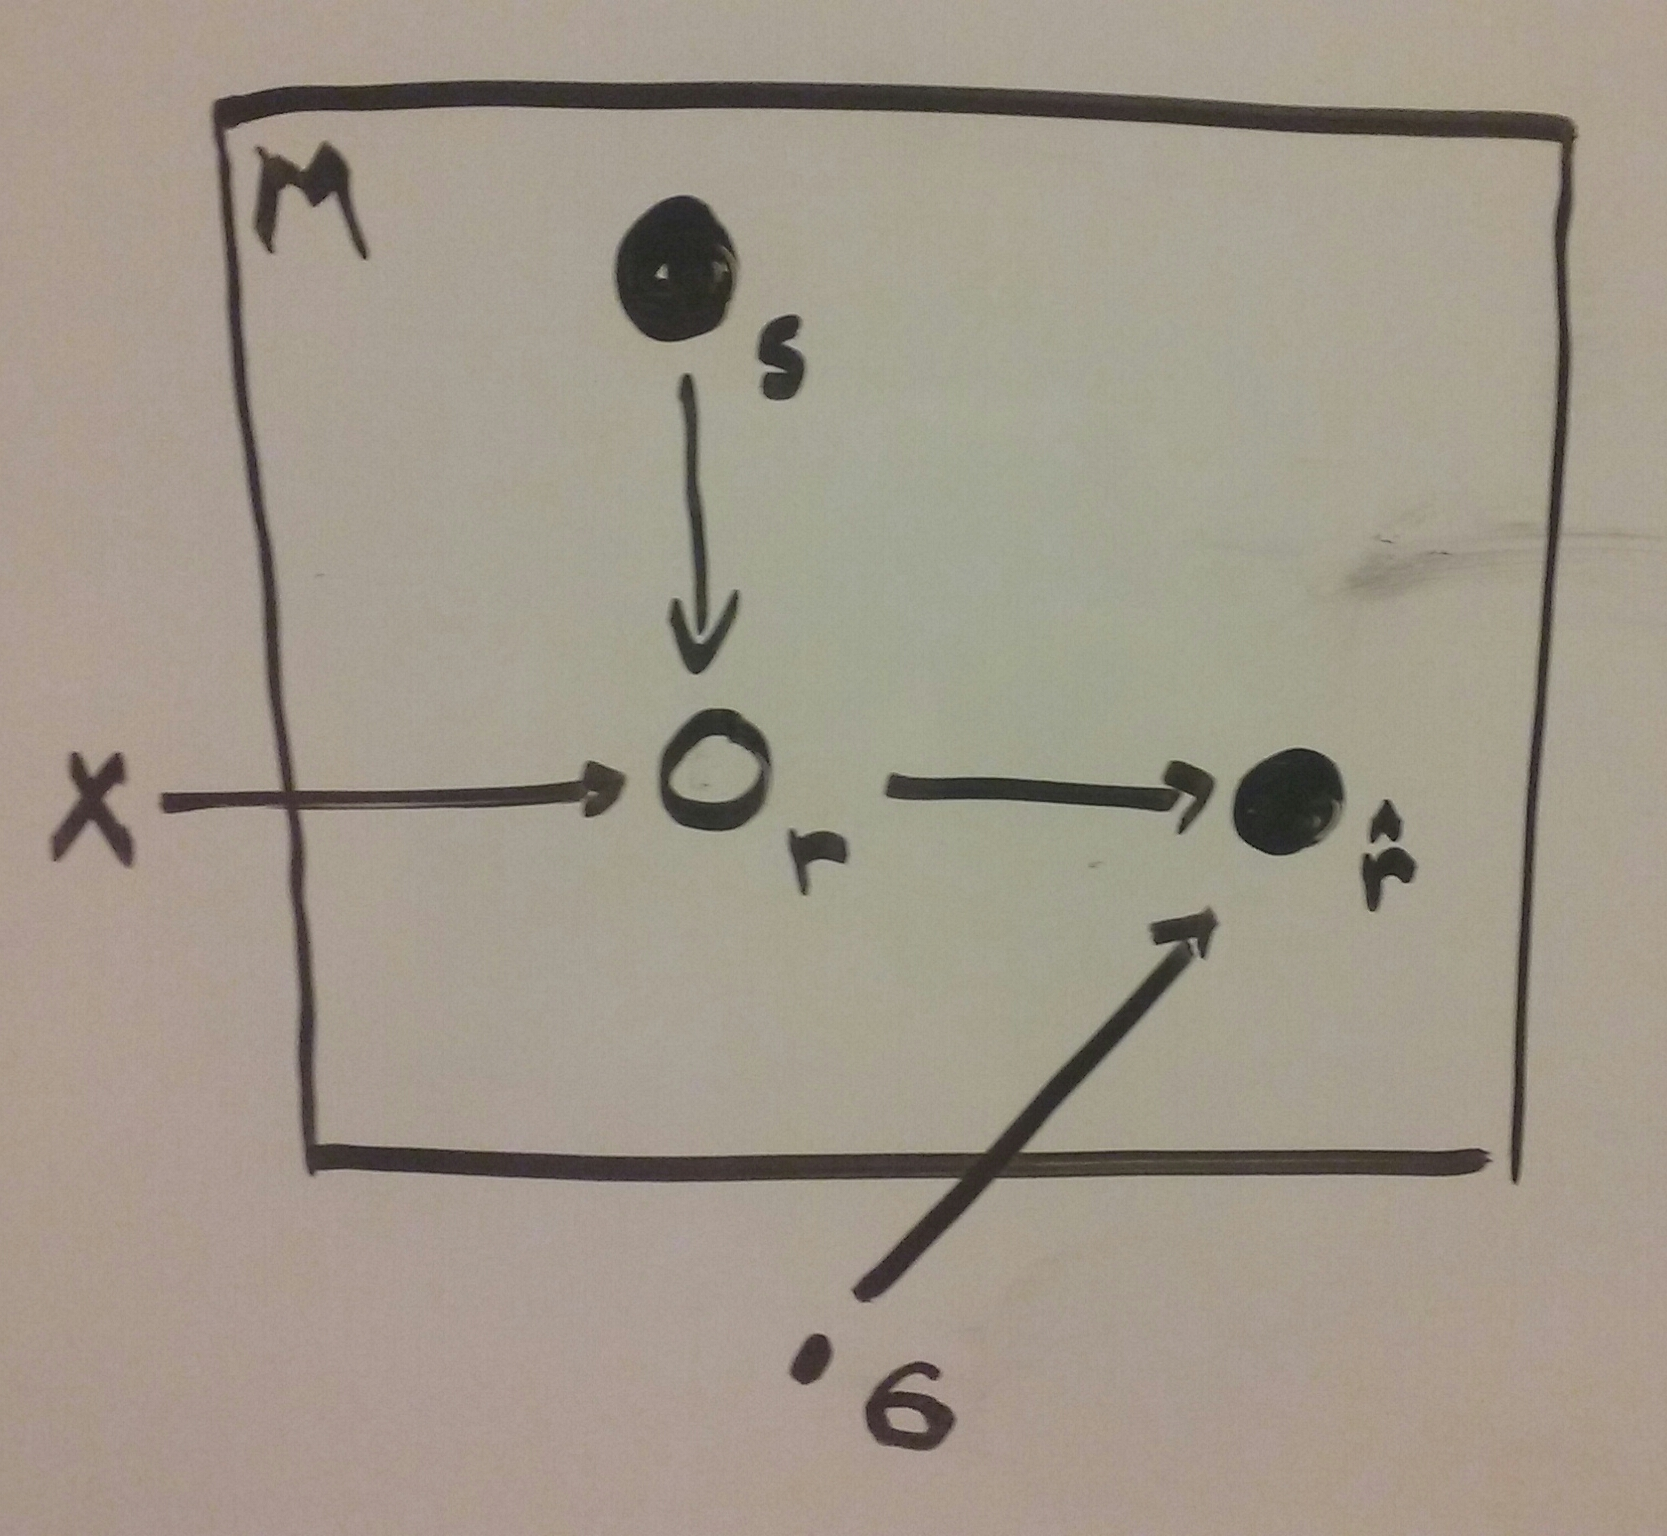
\includegraphics[height=1in]{pictures/1plate.jpg}

%abcd
\columnbreak

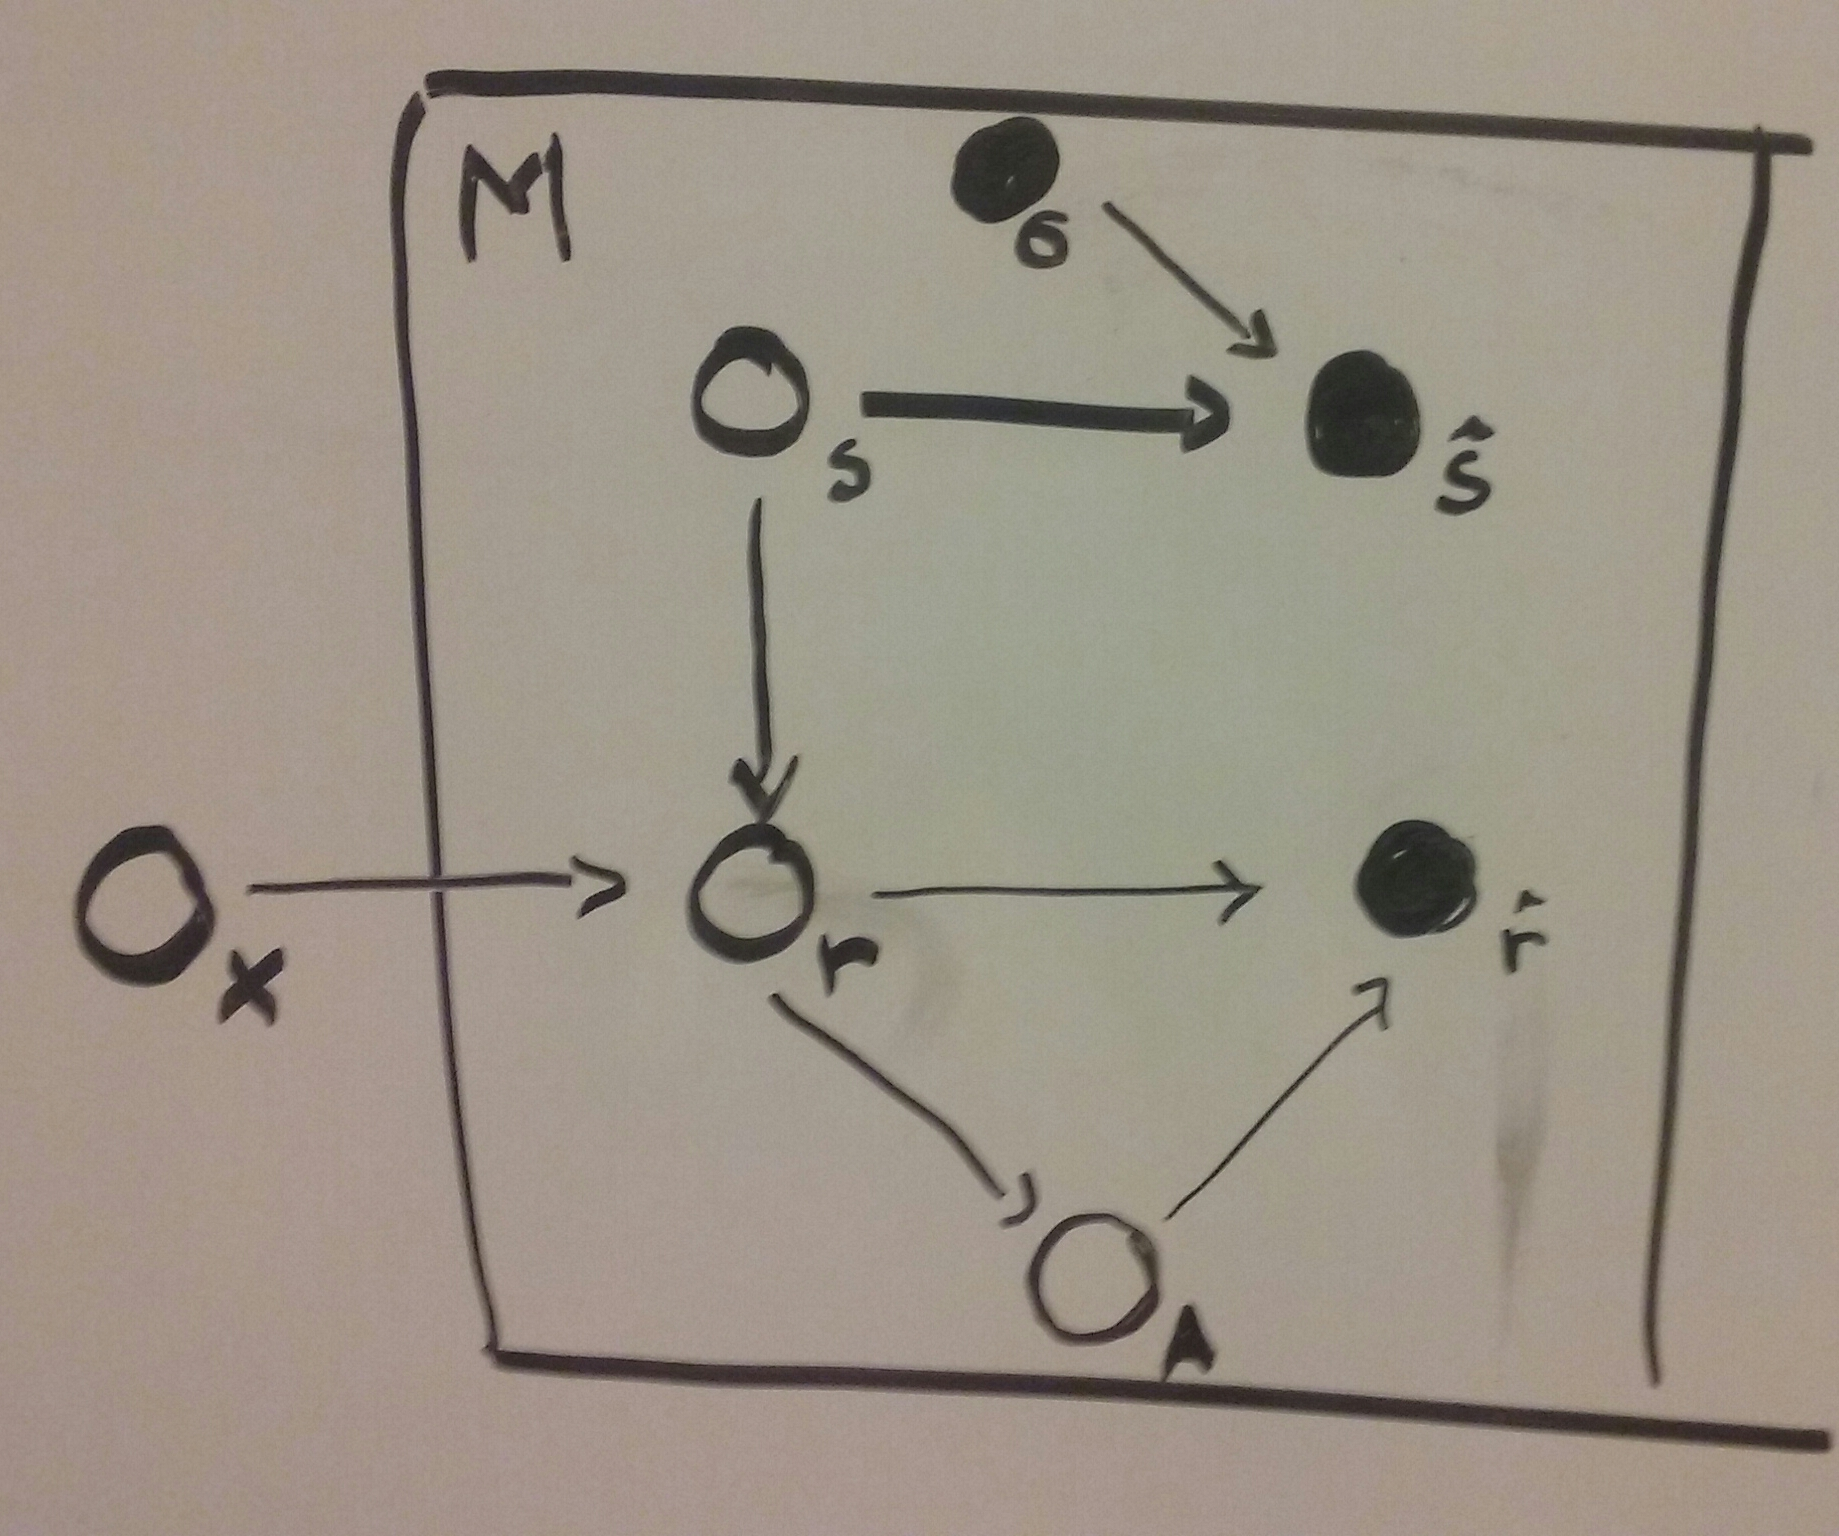
\includegraphics[height=1in]{pictures/2plate.jpg}

%abcd
\columnbreak

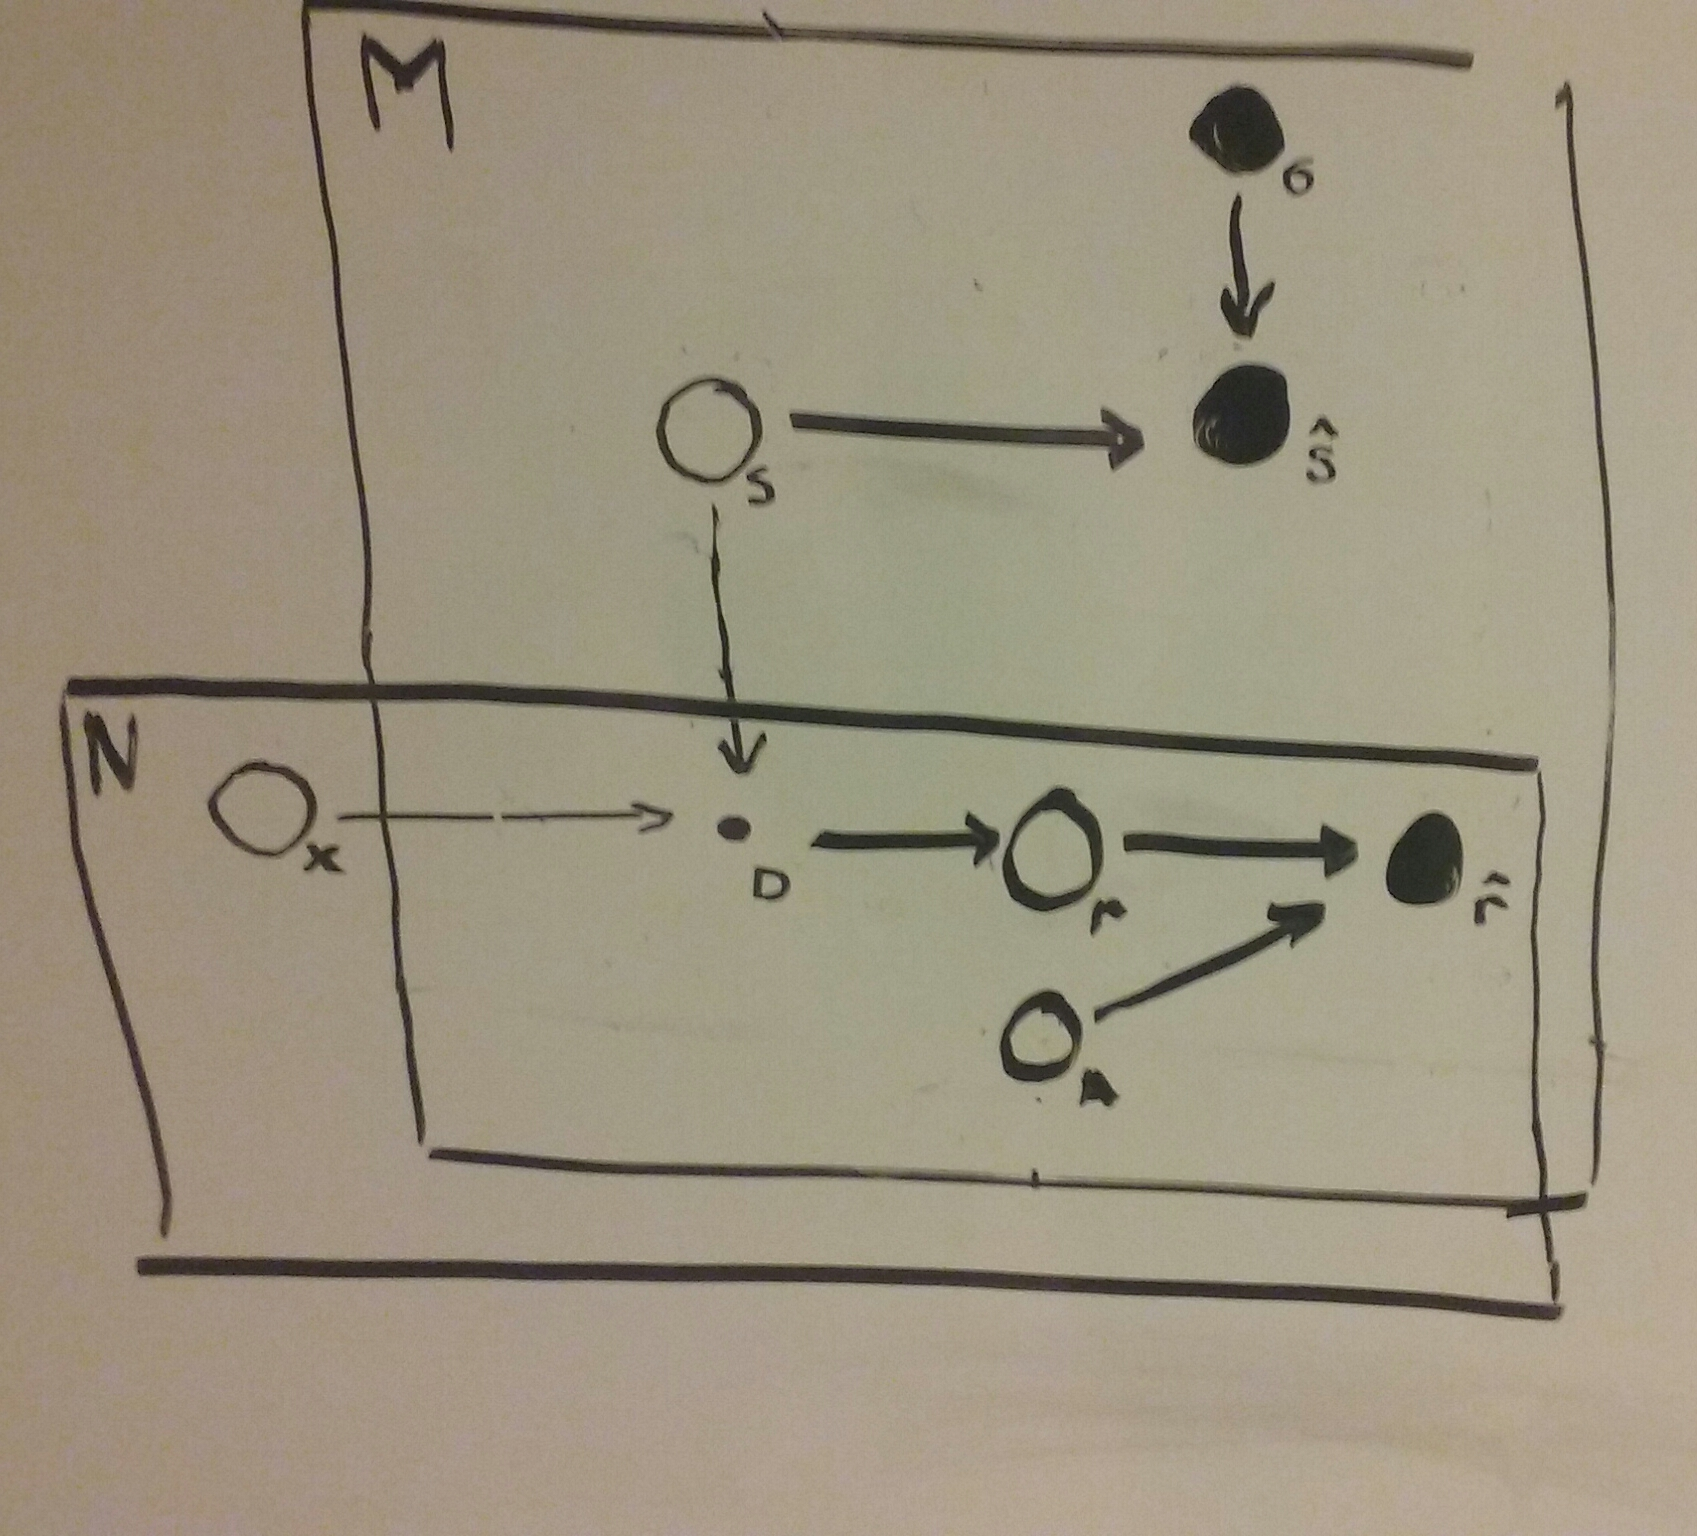
\includegraphics[height=1in]{pictures/3plate.jpg}

%abcd
\columnbreak
\end{multicols}
\end{center}
\begin{itemize}
\item[N] Transmitters
\item[M] Recievers
\item[S] Reciever Position
\item[X] Reciever Position
\item[r] Power
\item[A] Attinuation
\item[D] Distance
\end{itemize}

\end{frame}

\begin{frame}{Implementation - Supporting Technology}

    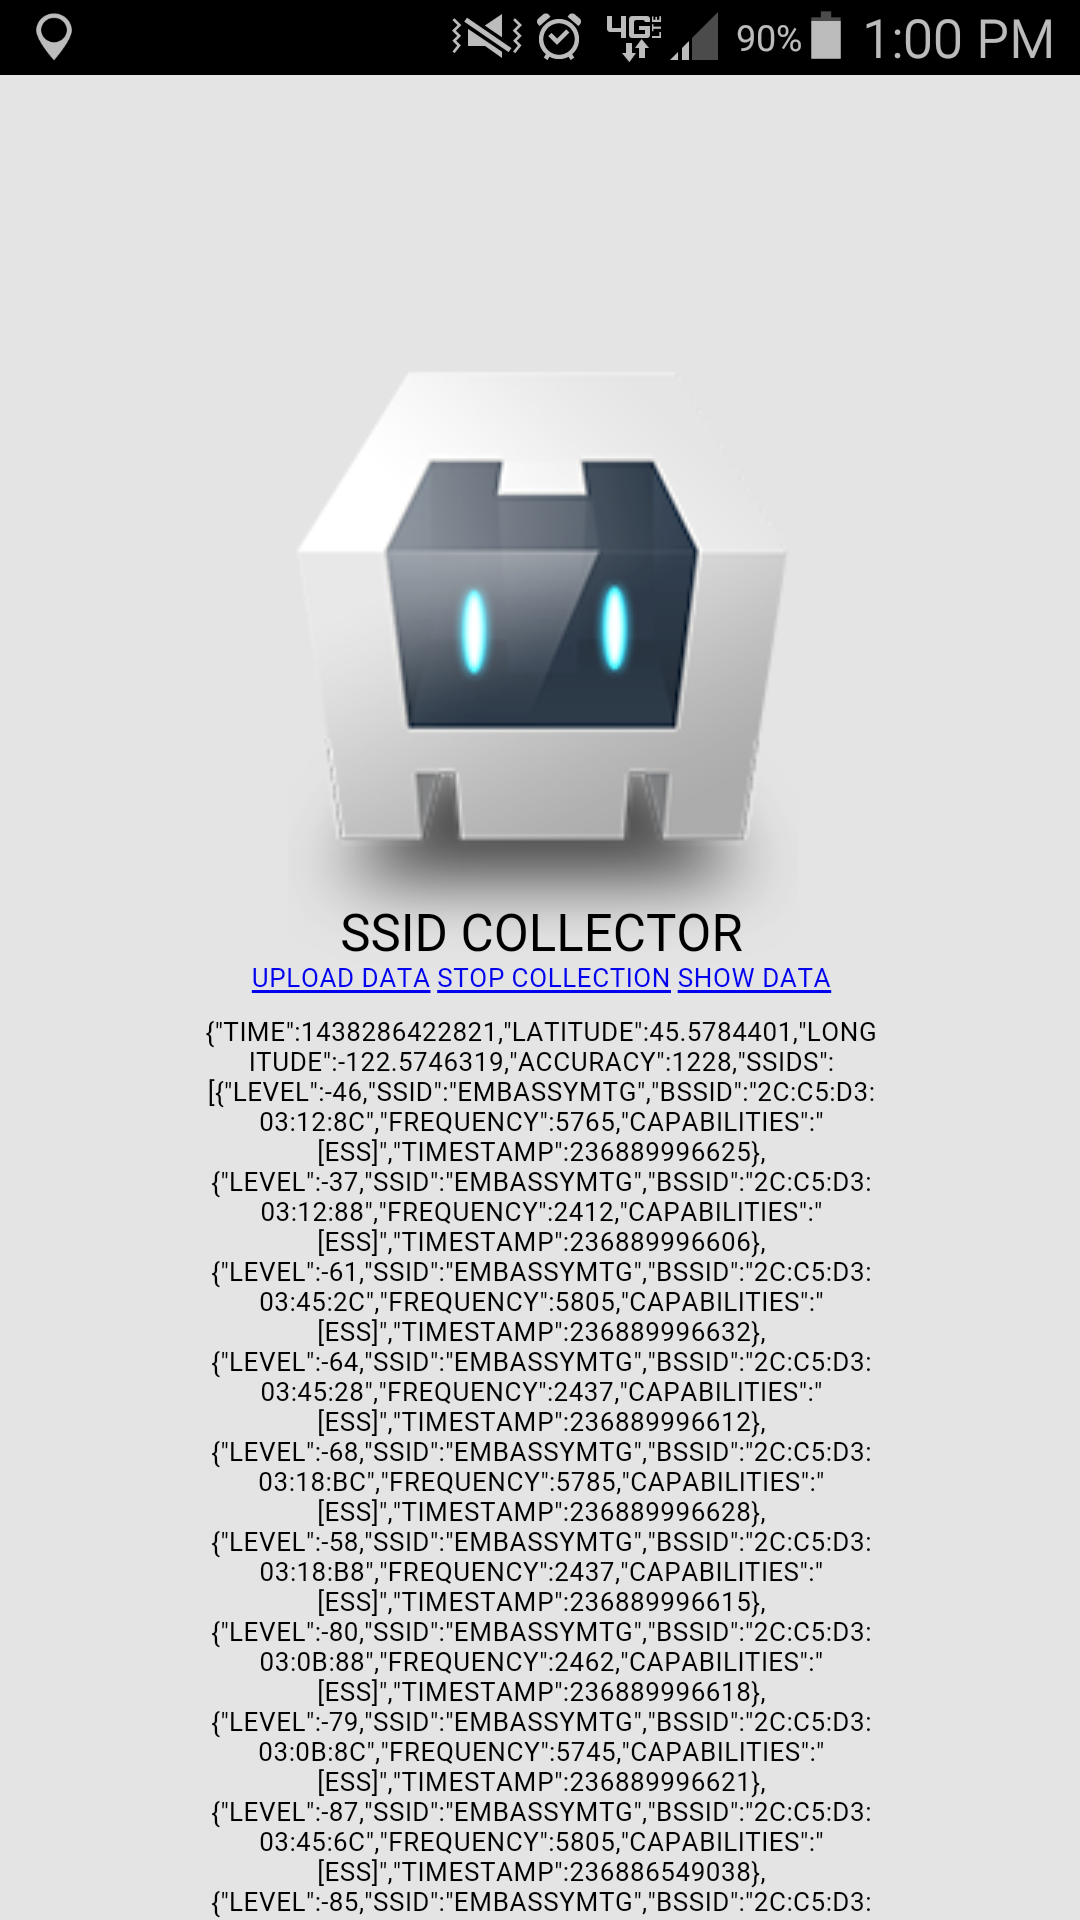
\includegraphics[height=0.7\textheight]{pictures/phoneapp.png}
    \begin{itemize}
        \item Phone app - Apache Cordova
        \item Backend - Couchdb
    \end{itemize}

\end{frame}

\begin{frame}{Visualization}

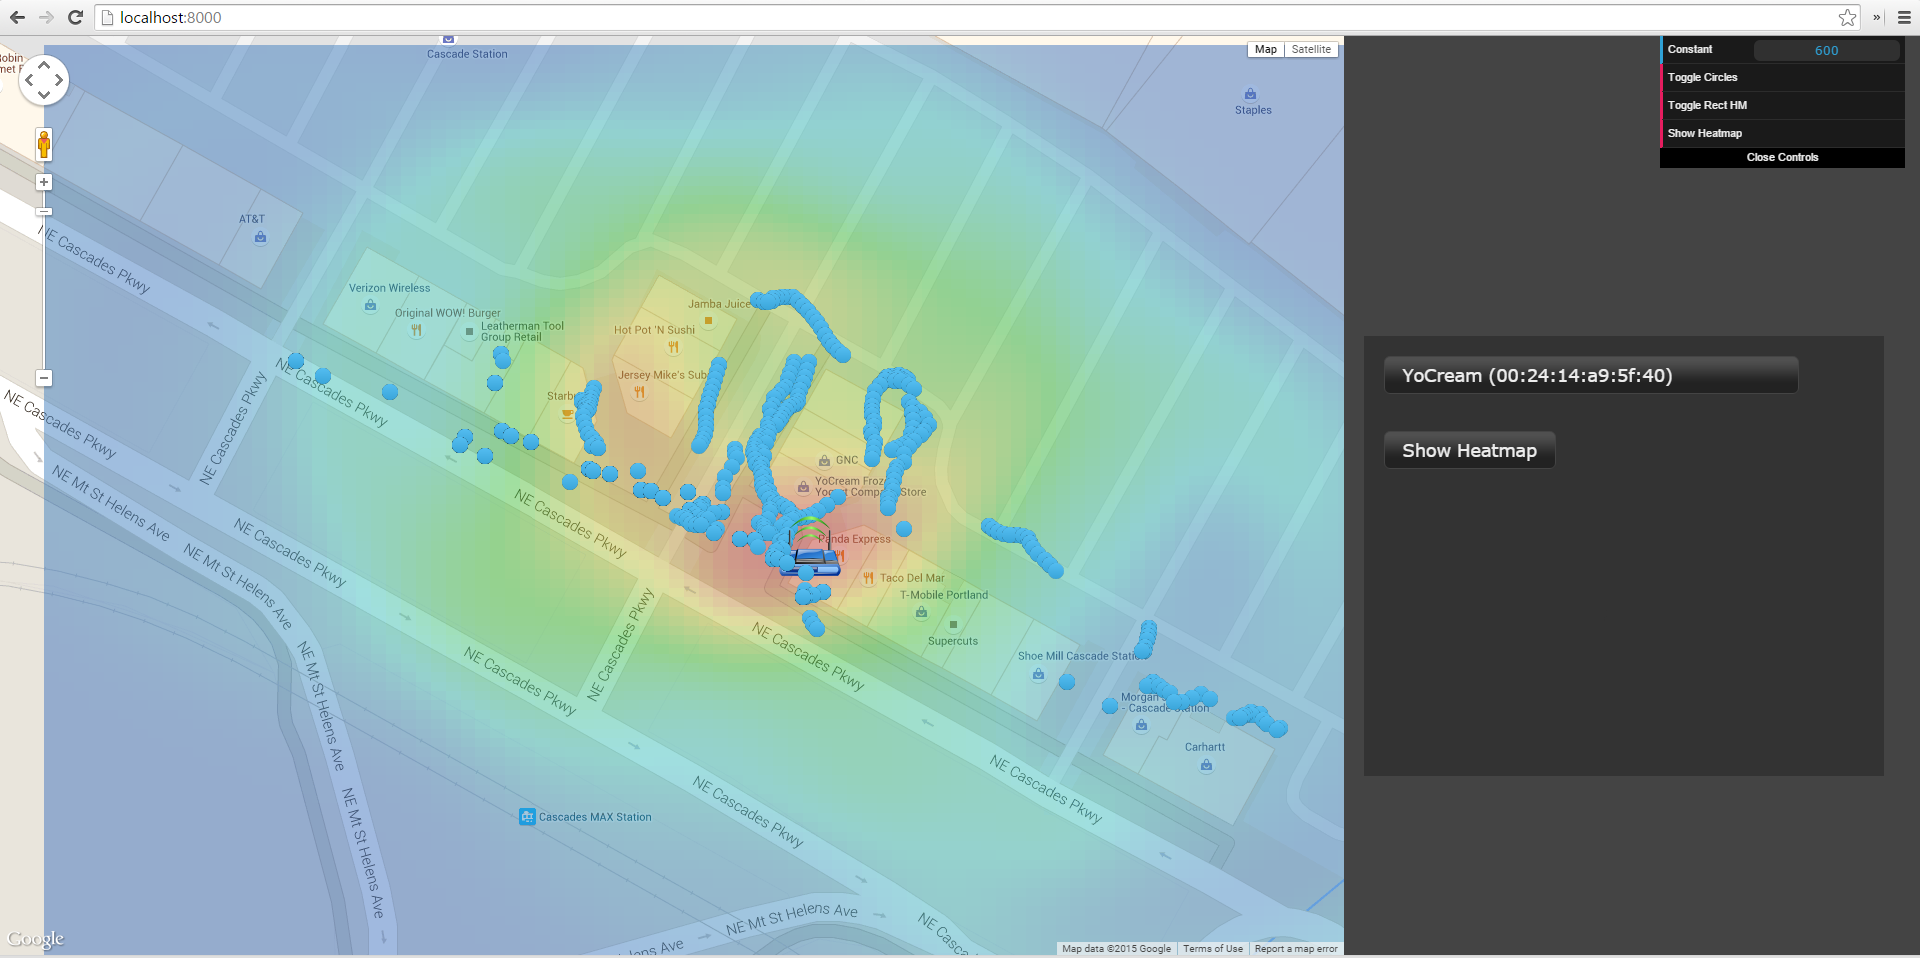
\includegraphics[height=0.7\textheight]{pictures/screenshot4.png}
\end{frame}

\begin{frame}{Implementation - Figaro}
\begin{multicols}{2}
\resizebox{!}{1.5in}{\lstinputlisting[
    basicstyle=\footnotesize,
    numbers=left,
    numberstyle=\tiny\color{gray}
  ]{probinso.scala}
}
\columnbreak

Hello
\end{multicols}

\end{frame}

\begin{frame}{Insights}

\end{frame}

\begin{frame}{Collateral}

\end{frame}

\end{document}
